%% File list of work: IEEEtran.cls, IEEEtran_HOWTO.pdf, bare_adv.tex,
%%                    bare_conf.tex, bare_jrnl.tex, bare_jrnl_compsoc.tex
% Some very useful LaTeX packages include:
% (uncomment the ones you want to load)


% *** MISC UTILITY PACKAGES ***
%
%\usepackage{ifpdf}
% Heiko Oberdiek's ifpdf.sty is very useful if you need conditional
% compilation based on whether the output is pdf or dvi.
% usage:
% \ifpdf
%   % pdf code
% \else
%   % dvi code
% \fi
% The latest version of ifpdf.sty can be obtained from:
% http://www.ctan.org/tex-archive/macros/latex/contrib/oberdiek/
% Also, note that IEEEtran.cls V1.7 and later provides a builtin
% \ifCLASSINFOpdf conditional that works the same way.
% When switching from latex to pdflatex and vice-versa, the compiler may
% have to be run twice to clear warning/error messages.






% *** CITATION PACKAGES ***
%
%\usepackage{cite}
% cite.sty was written by Donald Arseneau
% V1.6 and later of IEEEtran pre-defines the format of the cite.sty package
% \cite{} output to follow that of IEEE. Loading the cite package will
% result in citation numbers being automatically sorted and properly
% "compressed/ranged". e.g., [1], [9], [2], [7], [5], [6] without using
% cite.sty will become [1], [2], [5]--[7], [9] using cite.sty. cite.sty's
% \cite will automatically add leading space, if needed. Use cite.sty's
% noadjust option (cite.sty V3.8 and later) if you want to turn this off.
% cite.sty is already installed on most LaTeX systems. Be sure and use
% version 4.0 (2003-05-27) and later if using hyperref.sty. cite.sty does
% not currently provide for hyperlinked citations.
% The latest version can be obtained at:
% http://www.ctan.org/tex-archive/macros/latex/contrib/cite/
% The documentation is contained in the cite.sty file itself.






% *** GRAPHICS RELATED PACKAGES ***
%\ifCLASSINFOpdf
   %\usepackage[pdftex]{graphicx}
  % declare the path(s) where your graphic files are
  % \graphicspath{{../pdf/}{../jpeg/}}
  % and their extensions so you won't have to specify these with
  % every instance of \includegraphics
  % \DeclareGraphicsExtensions{.pdf,.jpeg,.png}
%\else
  % or other class option (dvipsone, dvipdf, if not using dvips). graphicx
  % will default to the driver specified in the system graphics.cfg if no
  % driver is specified.
  % \usepackage[dvips]{graphicx}
  % declare the path(s) where your graphic files are
  % \graphicspath{{../eps/}}
  % and their extensions so you won't have to specify these with
  % every instance of \includegraphics
  % \DeclareGraphicsExtensions{.eps}
%\fi
% graphicx was written by David Carlisle and Sebastian Rahtz. It is
% required if you want graphics, photos, etc. graphicx.sty is already
% installed on most LaTeX systems. The latest version and documentation can
% be obtained at: 
% http://www.ctan.org/tex-archive/macros/latex/required/graphics/
% Another good source of documentation is "Using Imported Graphics in
% LaTeX2e" by Keith Reckdahl which can be found as epslatex.ps or
% epslatex.pdf at: http://www.ctan.org/tex-archive/info/
%
% latex, and pdflatex in dvi mode, support graphics in encapsulated
% postscript (.eps) format. pdflatex in pdf mode supports graphics
% in .pdf, .jpeg, .png and .mps (metapost) formats. Users should ensure
% that all non-photo figures use a vector format (.eps, .pdf, .mps) and
% not a bitmapped formats (.jpeg, .png). IEEE frowns on bitmapped formats
% which can result in "jaggedy"/blurry rendering of lines and letters as
% well as large increases in file sizes.
%
% You can find documentation about the pdfTeX application at:
% http://www.tug.org/applications/pdftex





% *** MATH PACKAGES ***
%
%\usepackage[cmex10]{amsmath}
% A popular package from the American Mathematical Society that provides
% many useful and powerful commands for dealing with mathematics. If using
% it, be sure to load this package with the cmex10 option to ensure that
% only type 1 fonts will utilized at all point sizes. Without this option,
% it is possible that some math symbols, particularly those within
% footnotes, will be rendered in bitmap form which will result in a
% document that can not be IEEE Xplore compliant!
%
% Also, note that the amsmath package sets \interdisplaylinepenalty to 10000
% thus preventing page breaks from occurring within multiline equations. Use:
%\interdisplaylinepenalty=2500
% after loading amsmath to restore such page breaks as IEEEtran.cls normally
% does. amsmath.sty is already installed on most LaTeX systems. The latest
% version and documentation can be obtained at:
% http://www.ctan.org/tex-archive/macros/latex/required/amslatex/math/





% *** SPECIALIZED LIST PACKAGES ***
%
%\usepackage{algorithmic}
% algorithmic.sty was written by Peter Williams and Rogerio Brito.
% This package provides an algorithmic environment fo describing algorithms.
% You can use the algorithmic environment in-text or within a figure
% environment to provide for a floating algorithm. Do NOT use the algorithm
% floating environment provided by algorithm.sty (by the same authors) or
% algorithm2e.sty (by Christophe Fiorio) as IEEE does not use dedicated
% algorithm float types and packages that provide these will not provide
% correct IEEE style captions. The latest version and documentation of
% algorithmic.sty can be obtained at:
% http://www.ctan.org/tex-archive/macros/latex/contrib/algorithms/
% There is also a support site at:
% http://algorithms.berlios.de/index.html
% Also of interest may be the (relatively newer and more customizable)
% algorithmicx.sty package by Szasz Janos:
% http://www.ctan.org/tex-archive/macros/latex/contrib/algorithmicx/




% *** ALIGNMENT PACKAGES ***
%
%\usepackage{array}
% Frank Mittelbach's and David Carlisle's array.sty patches and improves
% the standard LaTeX2e array and tabular environments to provide better
% appearance and additional user controls. As the default LaTeX2e table
% generation code is lacking to the point of almost being broken with
% respect to the quality of the end results, all users are strongly
% advised to use an enhanced (at the very least that provided by array.sty)
% set of table tools. array.sty is already installed on most systems. The
% latest version and documentation can be obtained at:
% http://www.ctan.org/tex-archive/macros/latex/required/tools/


%\usepackage{mdwmath}
%\usepackage{mdwtab}
% Also highly recommended is Mark Wooding's extremely powerful MDW tools,
% especially mdwmath.sty and mdwtab.sty which are used to format equations
% and tables, respectively. The MDWtools set is already installed on most
% LaTeX systems. The lastest version and documentation is available at:
% http://www.ctan.org/tex-archive/macros/latex/contrib/mdwtools/


% IEEEtran contains the IEEEeqnarray family of commands that can be used to
% generate multiline equations as well as matrices, tables, etc., of high
% quality.


%\usepackage{eqparbox}
% Also of notable interest is Scott Pakin's eqparbox package for creating
% (automatically sized) equal width boxes - aka "natural width parboxes".

% Available at:
% http://www.ctan.org/tex-archive/macros/latex/contrib/eqparbox/





% *** SUBFIGURE PACKAGES ***
%\usepackage[tight,footnotesize]{subfigure}
% subfigure.sty was written by Steven Douglas Cochran. This package makes it
% easy to put subfigures in your figures. e.g., "Figure 1a and 1b". For IEEE
% work, it is a good idea to load it with the tight package option to reduce
% the amount of white space around the subfigures. subfigure.sty is already
% installed on most LaTeX systems. The latest version and documentation can
% be obtained at:
% http://www.ctan.org/tex-archive/obsolete/macros/latex/contrib/subfigure/
% subfigure.sty has been superceeded by subfig.sty.



%\usepackage[caption=false]{caption}
%\usepackage[font=footnotesize]{subfig}
% subfig.sty, also written by Steven Douglas Cochran, is the modern
% replacement for subfigure.sty. However, subfig.sty requires and
% automatically loads Axel Sommerfeldt's caption.sty which will override
% IEEEtran.cls handling of captions and this will result in nonIEEE style
% figure/table captions. To prevent this problem, be sure and preload
% caption.sty with its "caption=false" package option. This is will preserve
% IEEEtran.cls handing of captions. Version 1.3 (2005/06/28) and later 
% (recommended due to many improvements over 1.2) of subfig.sty supports
% the caption=false option directly:
%\usepackage[caption=false,font=footnotesize]{subfig}
%
% The latest version and documentation can be obtained at:
% http://www.ctan.org/tex-archive/macros/latex/contrib/subfig/
% The latest version and documentation of caption.sty can be obtained at:
% http://www.ctan.org/tex-archive/macros/latex/contrib/caption/




% *** FLOAT PACKAGES ***
%
%\usepackage{fixltx2e}
% fixltx2e, the successor to the earlier fix2col.sty, was written by
% Frank Mittelbach and David Carlisle. This package corrects a few problems
% in the LaTeX2e kernel, the most notable of which is that in current
% LaTeX2e releases, the ordering of single and double column floats is not
% guaranteed to be preserved. Thus, an unpatched LaTeX2e can allow a
% single column figure to be placed prior to an earlier double column
% figure. The latest version and documentation can be found at:
% http://www.ctan.org/tex-archive/macros/latex/base/



%\usepackage{stfloats}
% stfloats.sty was written by Sigitas Tolusis. This package gives LaTeX2e
% the ability to do double column floats at the bottom of the page as well
% as the top. (e.g., "\begin{figure*}[!b]" is not normally possible in
% LaTeX2e). It also provides a command:
%\fnbelowfloat
% to enable the placement of footnotes below bottom floats (the standard
% LaTeX2e kernel puts them above bottom floats). This is an invasive package
% which rewrites many portions of the LaTeX2e float routines. It may not work
% with other packages that modify the LaTeX2e float routines. The latest
% version and documentation can be obtained at:
% http://www.ctan.org/tex-archive/macros/latex/contrib/sttools/
% Documentation is contained in the stfloats.sty comments as well as in the
% presfull.pdf file. Do not use the stfloats baselinefloat ability as IEEE
% does not allow \baselineskip to stretch. Authors submitting work to the
% IEEE should note that IEEE rarely uses double column equations and
% that authors should try to avoid such use. Do not be tempted to use the
% cuted.sty or midfloat.sty packages (also by Sigitas Tolusis) as IEEE does
% not format its papers in such ways.





% *** PDF, URL AND HYPERLINK PACKAGES ***
%
%\usepackage{url}
% url.sty was written by Donald Arseneau. It provides better support for
% handling and breaking URLs. url.sty is already installed on most LaTeX
% systems. The latest version can be obtained at:
% http://www.ctan.org/tex-archive/macros/latex/contrib/misc/
% Read the url.sty source comments for usage information. Basically,
% \url{my_url_here}.





% *** Do not adjust lengths that control margins, column widths, etc. ***
% *** Do not use packages that alter fonts (such as pslatex).         ***
% There should be no need to do such things with IEEEtran.cls V1.6 and later.
% (Unless specifically asked to do so by the journal or conference you plan
% to submit to, of course. )


\documentclass[10pt, conference, compsocconf]{IEEEtran}
% \documentclass[conference]{../sty/IEEEtran}
\usepackage{graphicx}
\graphicspath{C:/Users/Megha/Desktop/SEM4/DDM/CourseProject/Documentation/ProjectReport_MT11024/}
\DeclareGraphicsExtensions{.pdf,.jpeg,.png}

% correct bad hyphenation here
\hyphenation{op-tical net-works semi-conduc-tor}

\begin{document}

\title{Evaluation of OCR Text Correction by\\
	 Crowdsourcing on a Historic Newspaper Archive}

\author{\IEEEauthorblockN{Megha Gupta and Haimonti Dutta*}
\IEEEauthorblockA{Department of Computer Science, IIIT-Delhi\\
**Affiliated to The Center for Computational Learning Systems, Columbia University, New York\\
(megha1124, haimonti)@iiitd.ac.in}
}

% make the title area
\maketitle

\begin{abstract}

Optical Character Recognition (OCR) is a common method of digitizing printed texts so that they can be electronically searched, stored compactly, displayed on-line, and used in text mining applications.\\
The text generated from OCR devices, however, is often garbled due to variations in quality of the input paper, size and style of the font and column layout. This adversely affects retrieval effectiveness and techniques for cleaning the OCR need to be improvised. Often such techniques involve laborious and time consuming manual processing of data.\\
This project deals with a subset of historical newspaper articles in the holdings of the California Digital Newspaper Collection \cite{cdnc} which have been OCR-ed. Patrons of the \cite{cdnc} read the Amador Ledger on a regular basis and correct OCR errors as they come across them.\\
This work can be used to determine whether the OCR text is clean enough to be used for thorough text search. The creation and analysis of this corpus will enable advanced search mechanisms on these holdings making them more
useful to the general public.\\

\end{abstract}

\begin{IEEEkeywords}
OCR; newspapers; historic; crowdsourcing;
\end{IEEEkeywords}

\section{Introduction}
The electronic conversion of scanned images of handwritten or printed text into a machine encoded text is widely done using Optical Character Recognition devices.  It finds most successful applications in the field of machine Learning, Artificial Intelligence and Pattern recognition.\\
OCR deals with the problem of recognising optically generated characters be it offline or online. Its performance directly depends on the quality of input document. The more constrained the input is the better will be the performance of the system. But when it comes to unconstrained handwriting, the performance is far from satisfactory.\\
The main application areas for \cite{OCR} like Automatic number plate readers, form readers, Signature verification and identification fall into three categories that is Data Entry, Text Entry, process automation.\\
This project deals with printed text in the form of Historical Newspaper Articles in the holdings of \cite{cdnc}. One such newspaper, The Amador Ledger published in the early 1900s by the Amador Publishing Company appealed to the community's interests by covering issues unique to gold mining.\\ 
Patrons of the \cite{cdnc} continue to be interested in studying about the status of the local mining industry and consequently read the Amador Ledger on a regular basis even to this day and correct \cite{OCR} errors as they come across them.\\
The corrections made by the patrons generate logfiles that maintain the history of what users have edited which further helps in generating the Corrected OCR corpus for evaluation and analysis.\\
Experiments are performed on both the datasets using the same Query set. The ranked documents retrieved from both the sets are compared using a statistical measure called Spearman's Rank Order Correlation. It measures the strength of association between two ranked variables.\\
This work can be used to determine whether the OCR text is sufficient enough to be used for the thorough text search and analysis and does it meet the user expectation without actually enhancing and enriching the text.\\

\subsection{Project Participants}
This is an individual project.

\subsection{Datasets and Software Used}
\subsubsection{Logfiles}
Logfiles were generated using a third party software for user text correction issued by Digital Libraries Consulting \cite{digital}. Using this software, patrons could edit the incorrect text, producing a logfile in xml format containing tags like \\
\textless OldTextValue\textgreater largest Plant in the World.\textless/OldTextValue\textgreater \\ 
\textless NewTextValue\textgreater Largest Plant in the World.\textless/NewTextValue\textgreater \\
\begin{figure}[ht!]
\centering
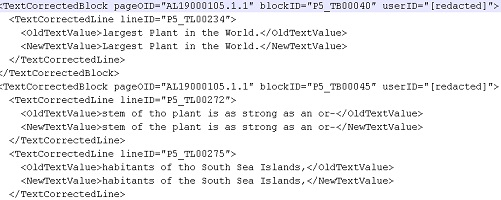
\includegraphics[width=9cm,height=5cm]{C:/Users/Megha/Desktop/SEM4/DDM/CourseProject/Documentation/ProjectReport_MT11024/logfile.jpg}
\caption{Log File}
\label{fig:Logfile}
\end{figure}

The names of the logfiles follow a convention as the first two letters represent the initials of the newspaper followed by the date as yyyymmdd.\\ For example AL19000105-changes.log includes Amador Ledger, 1900-01-05. There were in total 234 logfiles. \\

To get an idea of the number of corrections made by user per logfile, we created a histogram which is shown below. \\
\begin{figure}[ht!]
\centering
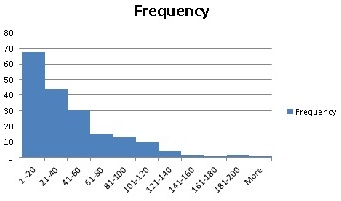
\includegraphics[width=9cm,height=5cm]{C:/Users/Megha/Desktop/SEM4/DDM/CourseProject/Documentation/ProjectReport_MT11024/histo.jpg}
\caption{Histogram}
\label{fig:histogram}
\end{figure}

The errors rectified by the users can be categorized as Spellcheck Error, Capitalization Error, Punctuation Error, Addition of new words, Omission of Garbled Text, etc.\\
\begin{figure}[h]
\centering
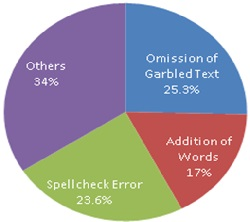
\includegraphics[width=3cm,height=3cm]{C:/Users/Megha/Desktop/SEM4/DDM/CourseProject/Documentation/ProjectReport_MT11024/stats.jpg}
\caption{Error Classification}
\label{fig:Statistics}
\end{figure}


\subsubsection{Raw OCR corpus}
This corpus had 190 files with the original OCR-ed text. It contains errors due to inaccurate conversion from printed to digitized text by OCR devices. The files in this corpus were extracted from the the website \cite{datasource} using Python scripts. The general idea was to decode the names of the logfiles to get the name and date of the newspaper. Further these name and dates were formulated into a URL. The url for a particular issues has a pattern that changes only with the date of the issue. The issue we dealt with in our corpus was Amador Ledger, ranging from 1900-01-05 to 1910-12-30.  For instance, AL19000105-changes.log was converted to Amador Ledger, 1900-01-05 which was further translated to http://chroniclingamerica.loc.gov/lccn/sn93052980/1900-01-05/ed-1/seq-1/ocr.txt\\

\subsubsection{Corrected OCR Corpus}
This corpus incorporated users corrections that were recorded in logfiles. It was generated by replacing the old text in the Raw OCR corpus with the new text given in the logfiles. Python scripts were used to integrate both the datasets, that are the logfiles and the Raw corpus to create a new Corrected corpus containing 190 files.\\

\subsubsection{Query Set}
This dataset was created by randomly picking words only from the Corrected corpus as this corpus is an enhanced copy of Raw Corpus. So the keywords include ocr-ed text that was not touched by the patrons and the text that was corrected by them through crowd sourcing. \\

\subsubsection {Software}
PyLucene 3.6.2, a Python extension for accessing Java Apache Lucene was used as an IR software library for enabling full text indexing and searching capabilites. Inverted Index was built on each corpus with the fields stored as file name, file path and file contents making retrieval faster.

\section{Problem Statement}
This research is primarily focussed on retrieval effectiveness of OCR data versus Corrected data. We are trying to figure out what are the effects of noisy data on text retrieval. To know the difference between the results we need to find a heuristic measure that determines the difference between the retrieval effictiveness of OCR data versus Corrected Data. The aim of the project is to create and analyse the corrected OCR corpus using a metric that would measure the difference between the retrieval effectiveness of both the corpora, that is Raw OCR versus Corrected OCR.

\section{Methodology}
\subsection{Preprocessing \& Data Generation}
\subsubsection{Logfiles} Downloaded the Logfiles from the file server using pscp command. These Logfiles (xml format) maintain the history of old OCR text between the tag \textless OldTextValue\textgreater \textless/OldTextValue\textgreater \\ 
 and corresponding corrected text between \textless NewTextValue\textgreater \textless/NewTextValue\textgreater \space tag. \\

\subsubsection{Raw OCR Corpus}
These logfile names were decoded into Newspaper name  and Date of Newspaper. \\
For example, Logfile name, AL19000105-changes.log was converted to Amador Ledger, 1900-01-05 \\
Then each of the decoded name was translated into eight individual URLs.\\
http://chroniclingamerica.loc.gov/lccn/sn93052980/1900-01-05/ed-1/seq-1/ocr.txt\\
http://chroniclingamerica.loc.gov/lccn/sn93052980/1900-01-05/ed-1/seq-2/ocr.txt\\
http://chroniclingamerica.loc.gov/lccn/sn93052980/1900-01-05/ed-1/seq-3/ocr.txt\\
http://chroniclingamerica.loc.gov/lccn/sn93052980/1900-01-05/ed-1/seq-4/ocr.txt\\
http://chroniclingamerica.loc.gov/lccn/sn93052980/1900-01-05/ed-1/seq-5/ocr.txt\\
http://chroniclingamerica.loc.gov/lccn/sn93052980/1900-01-05/ed-1/seq-6/ocr.txt\\
http://chroniclingamerica.loc.gov/lccn/sn93052980/1900-01-05/ed-1/seq-7/ocr.txt\\
http://chroniclingamerica.loc.gov/lccn/sn93052980/1900-01-05/ed-1/seq-8/ocr.txt\\
where seq-1 represents the sequence of the pages of the newspaper.
Finally, we downloaded the Raw OCR text from each of these URLs from \cite{datasource} with the help of Python scripts to build the Raw OCR corpus.\\

\subsubsection{Corrected OCR Corpus}
Replacing the incorrect text with the corrected text from the logfiles in the Raw OCR Corpus, we obtain the Corrected OCR Corpus. The old and its corresponding new text were stored as key value pairs of a dictionary. Once all the pairs were generated from a log file, the text from the Raw Corpus matching with keys of the dictionary was replaced with the values corresponding to the matched key. \\

\subsection{Building IR Model}
PyLucene, is a wrapper around Java Lucene that allows full functionality of  lucene in Python. Its goal is to allow the use of Lucene's text indexing and searching capabilities from Python.\\
We have used PyLucene 3.6.2 in the project for Indexing and retrieving documents. Firstly, inverted indexes were created for both the datasets. An Inverted Index is an inside out arrangement of documents where terms take the center stage and each term points to a list of documents that contain it. Index file  contain fields, that includes, file name, file path and content.\\
Lucene's logical View of Index files features segments which contain indexed documents. Segments can be searched independently and the number of segments are determined by the number of documents to be indexed and the maximum number of documents in each segment.\\
\subsection{Query Set generation}
The Query set was formulated by randomly picking keywords from each of the Corrected OCR document. Each Query comprise of a single word keyword, for example "bapism", "eparmen", "elecors", etc. The number of keywords in the query set is around 200.
\subsection{Experimentation}
The experiments were run on the indexes created on both the datasets using the same query set. Once the query set was generated, it was passed through the searching script that retrieves the documents containing the keywords.\\
 The documents retrieved are ranked according to the frequency of the keyword present in the document. Higher the frequency, higher the ranking order.\\

\subsection{Results}
The ranked retrieved results (documents) from both the corpus for a query "January" are shown below : \\
From Corrected OCR \\

Top 10 matching Documents \\
name:1900-01-12.txt \\
name:1902-01-17.txt \\
name:1900-01-05.txt \\
name:1904-01-08.txt \\
name:1905-01-27.txt \\
name:1902-02-07.txt \\
name:1904-01-29.txt \\
name:1904-12-30.txt \\
name:1905-01-13.txt \\
name:1908-08-14.txt \\

From Raw OCR \\

Top 5 matching Documents \\
name:1900-01-12.txt \\
name:1902-01-17.txt \\
name:1900-01-05.txt \\ 
name:1904-01-08.txt \\
name:1905-01-13.txt \\



\subsection{Evaluation}
The metric we used to compare the ranked retrieved documents is Spearman's rank correlation coefficient(P). It is a nonparametric measure of statistical dependence between two variables. It assesses how well the relationship between two variables can be described using a monotonic function. If there are no repeated data values, a perfect Spearman correlation of +1 or -1 occurs when each of the variables is a perfect monotone function of the other.\\
Spearman's coefficient, like any correlation calculation, is appropriate for both continuous and discrete variables, including ordinal variables.\\
In applications where duplicate values are not present, the spearman's coefficient can be calculated using the below formula.\\
The ranking order of the documents retrieved from the Corrected OCR Corpus ($Y_{i}$) is shown in Rank $y_{i}$ whereas the order for the Raw OCR ($X_{i}$) is given as Rank $x_{i}$ . When the retrieved documents from both the dataset differ, then ranking of the Corrected OCR will be treated as a benchmark and Raw OCR will be ranked according to it. But the actual rank of the Raw OCR will be the sorted order of the rank given in accordance with the benchmark. \\

Differences $d_{i}$ = $x_{i}$ - $y_{i}$  between the ranks of each observation on the two variables are calculated, and P is given by:
P = 1 - $\frac {6\sum d_i^2 }{n(n^2-1)}$ \\

Following table shows the evaluation of P for a single query "January" (Best Case).

\begin{tabular}{ l | c | c | c | r | r }
$Y_{i}$ & $X_{i}$ & Rank $y_{i}$ & Rank $x_{i}$ & $d_{i}$ & $d_{i}^2$ \\
\hline
  12-01-1900 & 12-01-1900 & 1 & 1 & 0 & 0 \\
  17-01-1902 & 17-01-1902 & 2 & 2 & 0 & 0 \\
  05-01-1900 & 05-01-1900 & 3 & 3 & 0 & 0 \\
  08-01-1904 & 08-01-1904 & 4 & 4 & 0 & 0 \\
  27-01-1905 & 13-01-1905 & 5 & 9(5) & 0 & 0 \\
\end{tabular}
\\
\\
${\sum d_i^2}$ = 0 \\
P = 1 - $\frac{6*0}{5*24}$ \\
P = 1 \\

For another Query "Jackson", the evaluation of P (Worst Case) is as follows:

\begin{tabular}{ l | c | c | c | r | r }
 $Y_{i}$ & $X_{i}$ & Rank $y_{i}$ & Rank $x_{i}$ & $d_{i}$ & $d_{i}^2$ \\
\hline
  12-01-1900 & 21-10-1910 & 1 & 10(4) & -3 & 9 \\
  09-12-1910 & 09-12-1910 & 2 & 2(1) & 0 & 0 \\
  08-06-1900 & 23-09-1910 & 3 & 7(2) & 1 & 1 \\
  01-04-1904 & 02-12-1910 & 4 & 8(3) & 1 & 1 \\
  25-05-1900 & 23-12-1910 & 5 & 11(5) & 0 & 0 \\
\end{tabular}
\\
\\
${\sum d_i^2}$ = 11 \\
P = 1 - $\frac{6*11}{5*24}$ \\
P = 0.45 \\

The average value of Spearman's ranked correlation cofficient can be determined by averaging the Best and Worst case. \\
P = $\frac {0.8+0.45}{2}$ = 0.625 \\



\section{Conclusion}
The sign of the Spearman correlation indicates the direction of association between X (Raw OCR results) and Y (Corrected OCR results). If Y tends to increase when X increases, the Spearman correlation coefficient is positive. If Y tends to decrease when X increases, the Spearman correlation coefficient is negative. A Spearman correlation of zero indicates that there is no tendency for Y to either increase or decrease when X increases. The Spearman correlation increases in magnitude as X and Y become closer to being perfect monotone functions of each other. When X and Y are perfectly monotonically related, the Spearman correlation coefficient becomes 1. \\
The average value of Spearman's ranked correlation coefficient calculated by our experiments is 0.625 which can be interpreted as the association between the two corpora is not very strong but the positive value shows that if Raw OCR increases then Corrected OCR will definitely increase.

To use F-measure we need to have the record of relevant documents for each query. Every user has its own notion of relevance as it is a subjective measure.\\



% conference papers do not normally have an appendix
\section{Future Work}
Due to lack of time, we could not incorporate the users feedback or judgement regarding relevant and non relevant documents for particular query. We would like to extend our evaluation using F-score. \\
Also, we would like to enhance our search capabilities from single word query to multiple words or phrases. \\


% use section* for acknowledgement
\section*{Acknowledgment}
I would like to express my gratitude to my Advisor, Dr. Haimonti Dutta for her support, patience and encouragement throughout the course of the project. \\

\nocite{datasource,cdnc,digital}

\section{Bibiliography}
\bibliography{Project_report}
\bibliographystyle{plain}

% that's all folks
\end{document}


